% hand_built.tex

\marginnote{beginning of models/hand\_built.tex}

\subsection{Build an interesting grammar by hand}
\marginnote{Should probably do hand here?}

\marginnote{Move this experiment to the section on building a grammar
  from a single curve.}

Here we are drawing a grammar. We have built this grammar by hand, by
taking the following curve, and specifying a decomposition of it:

\begin{figure}
\includegraphics[width=\linewidth]{experiments/1.grammars/hand_built/output.d/hand_built_curve.png}
\caption{The initial curve}
\end{figure}

Here is the decomposition:
\begin{figure}
\includegraphics[width=\linewidth]{experiments/1.grammars/hand_built/output.d/hand_built_sdf.png}
\end{figure}

Here is the grammar:

\begin{figure}
Here are some samples from the grammar:

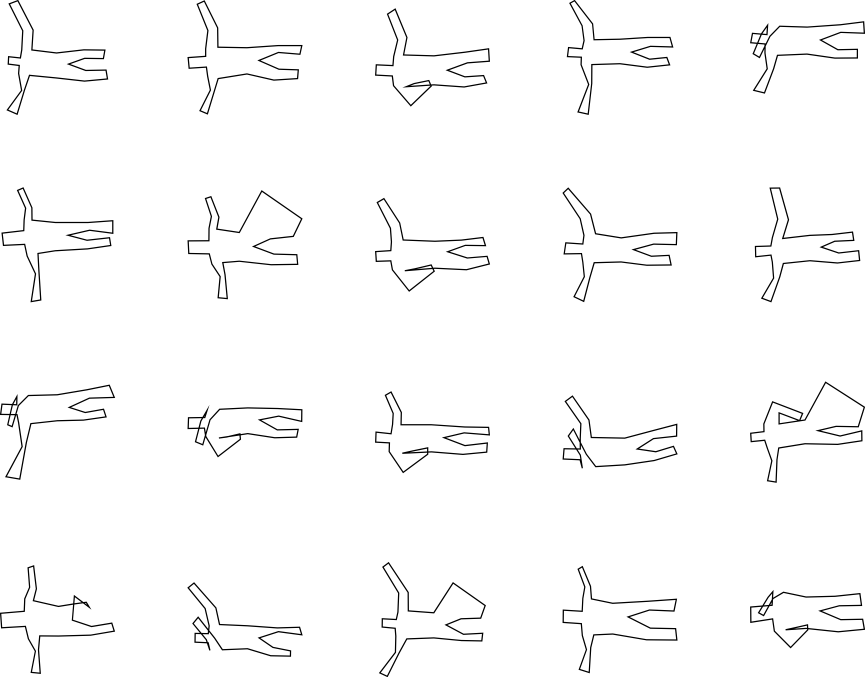
\includegraphics[width=6in]{output/3.learning/incremental/gram.19.d/samples.png}


\end{figure}

\marginnote{end of models/hand\_built.tex}
